%
% spinodal.tex -- Spinodale Entmischung
%
% (c) 2024 Patrik Müller, Hochschule Rapperswil
%
% !TeX root = ../../buch.tex
% !TeX encoding = UTF-8
% !TeX spellcheck = de_CH
%

\section{Spinodale Entmischung\label{cahnhilliard:section:spinodal}}
\kopfrechts{Spinodale Entmischung}
\index{spinodale Entmischung}%
Nachdem wir die Cahn-Hilliard-Gleichung hergeleitet haben,
möchten wir nun überprüfen,
ob \eqref{cahnhilliard:cheq} tatsächlich das Verhalten von Essig und Öl widerspiegelt.
Zu diesem Zweck wurde eine Simulation mit der Finite-Elemente-Methode (FEM) durchgeführt.
In der Simulation wurden die folgenden Parameter,
Funktionen und Anfangsbedingungen verwendet:
\begin{align*}
\begin{aligned}
M
&=
1,
&
\varepsilon
&=
0.01,
&
F(c)
&=
100 c^2 (c - 1)^2,
&
c(x,0)
&=
\frac{2}{3} + 0.01 X
,\; \text{wobei }
X
\sim
\mathcal{U}(-1,1)
.
\end{aligned}
\end{align*}
Dabei stellt $\mathcal{U}(-1,1)$ eine Gleichverteilung von $-1$ bis $1$ dar.
Für $c(x,0)$ wurde absichtlich das aus Kochbüchern typische Verhältnis von
\index{Kochbuch}%
2 Teile Öl zu 1 Teil Essig gewählt.
Wir nehmen ausserdem an, dass die Sauce initial sehr gut gemischt ist.
Der Code für die Simulation ist unter \cite{cahnhilliard:repo} abgelegt.

In Abbildung~\ref{cahnhilliard:fig:chsim} sind die Resultate der Simulation
zu verschiedenen Zeitpunkten dargestellt.
Man kann sehen,
wie sich das homogene Gemisch in seine einzelnen Komponenten zerlegt
und dabei eine Konfiguration
mit möglichst kleiner Grenzoberfläche zwischen den Phasen bildet.
Diese Simulation zeigt anschaulich die spinodale Entmischung,
bei der kleine Fluktuationen in der Konzentration zu einer Trennung der Phasen führen.

\begin{figure}
\centering
\foreach \n [count=\xi] \i in {0,5,10,15,25,50,80,130,300,1500,70000}{
%\subfigure[$t = \i\,\tau$]{
%\includegraphics[width=0.3\textwidth]{papers/cahnhilliard/presentation/images/ch_sim/\i.pdf}
%}
\begin{subfigure}{0.3\textwidth}
\includegraphics[width=\textwidth]{papers/cahnhilliard/presentation/images/ch_sim/\i.pdf}
\caption{$t = \i\,\tau$}
\end{subfigure}
}
%\subfigure[Farbskala]{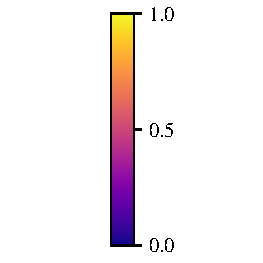
\includegraphics[width=0.3\textwidth]{papers/cahnhilliard/presentation/images/colorbar.book.pdf}}
\begin{subfigure}{0.3\textwidth}
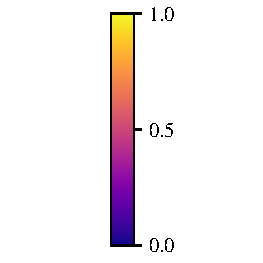
\includegraphics[width=\textwidth]{papers/cahnhilliard/presentation/images/colorbar.book.pdf}
\caption{Farbskala}
\end{subfigure}
\caption[Simulation der Cahn-Hilliard-Gleichung]{%
Simulation der Cahn-Hilliard-Gleichung und Entwicklung von $c(x,t)$ über einen langen Zeitraum.}
\label{cahnhilliard:fig:chsim}
\end{figure}

\subsection{Ursache für die Entmischung}

Die Phasentrennung in einem Gemisch wie Essig und Öl
ist ein faszinierendes physikalisches Phänomen,
das auf die grundlegenden Prinzipien der Thermodynamik zurückgeht.
Um zu verstehen,
warum sich zwei Flüssigkeiten wie Essig und Öl nicht mischen,
müssen wir die Konzepte der freien Energie und
der chemischen Potenziale näher betrachten.

In einem binären Gemisch wird die Gesamtenergie des Systems
durch die freie Energie $F(c)$ bestimmt,
die sowohl die inneren Wechselwirkungen der Moleküle
als auch die Entropie des Systems berücksichtigt.
Diese Funktion reflektiert die energetischen Kosten der Mischung der beiden Komponenten.
Die freie Energie für ein solches Gemisch kann laut \cite{cahnhilliard:deriv}
folgendermassen ausgedrückt werden:
\begin{align*}
F(c)
&=
\omega c (1 - c) + R T \left[ (1-c) \log(1-c) + c \log(c) \right].
\end{align*}
Hierbei ist $\omega$ ein Parameter,
der die Wechselwirkungsenergie zwischen den Komponenten beschreibt,
$R$ die universelle Gaskonstante und
\index{Gaskonstante}%
$T$ die Temperatur.
\index{Temperatur}%

Ein wesentlicher Aspekt ist die unterschiedliche chemische Affinität
der Moleküle zueinander.
Essig,
der hauptsächlich aus Wasser besteht,
und Öl haben sehr unterschiedliche molekulare Strukturen und Wechselwirkungen.
Wasser ist ein polares Molekül und bildet starke Wasserstoffbrückenbindungen,
\index{polar}%
\index{Wasserstoffbrückenbindung}%
während Öl aus unpolaren Kohlenwasserstoffmolekülen besteht,
\index{Kohlenwasserstoff}%
die keine solchen Bindungen eingehen.
Diese unterschiedlichen Wechselwirkungen führen dazu,
dass die Moleküle von Essig und Öl es vorziehen,
sich jeweils mit ihresgleichen zu umgeben,
anstatt sich miteinander zu vermischen.

\subsubsection{Kritische Temperatur}
\index{Temperatur!kritisch}%
Wenn wir die freie Energie $F(c)$ eines homogenen Gemisches analysieren,
stellen wir fest,
dass bei bestimmten Temperaturen die freie Energie eine Form annimmt,
die eine Mischung der Komponenten energetisch ungünstig macht.
Insbesondere bei Temperaturen unterhalb einer kritischen Temperatur $T_\text{krit}$
zeigt die freie Energie eine konkave Form im Bereich der mittleren Konzentrationen.
In Abbildung~\ref{cahnhilliard:fig:fc}
ist diese Temperaturabhängigkeit von $F(c)$ dargestellt.
Dies bedeutet,
dass das System energetisch bevorzugt ist,
sich in zwei Phasen mit unterschiedlichen Konzentrationen zu trennen,
um die Gesamtenergie zu minimieren.
Die kritische Temperatur kann durch die Beziehung
\begin{align*}
T_\text{krit}
&=
\frac{\omega}{2 R}
\end{align*}
bestimmt werden.

\begin{figure}
\centering
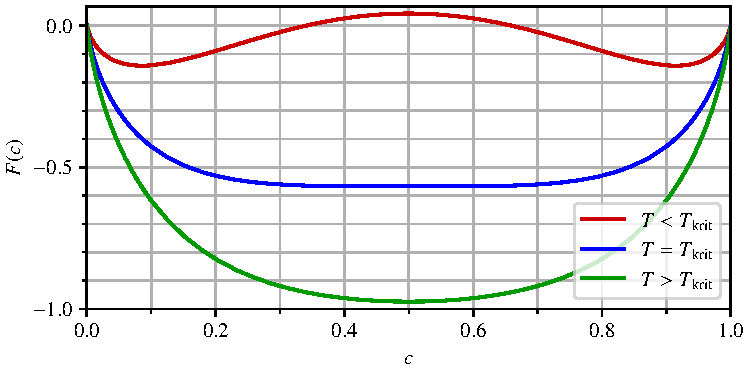
\includegraphics[scale=0.8]{papers/cahnhilliard/presentation/images/energy.book.pdf}
\caption{Temperaturabhängigkeit von $F(c)$.}
\label{cahnhilliard:fig:fc}
\end{figure}

Diese Trennung der Phasen wird durch kleine Fluktuationen in der Konzentration initiiert,
die durch thermische Bewegungen der Moleküle verursacht werden.
Sobald diese Fluktuationen auftreten,
führt die minimierte freie Energie dazu,
dass sich die Phasen weiter trennen und stabile Bereiche hoher
und niedriger Konzentration bilden.
Dieser Prozess wird als spinodale Entmischung bezeichnet
und beschreibt die spontane Bildung von Phasen,
die in der Cahn-Hilliard-Gleichung \eqref{cahnhilliard:cheq} modelliert wird.

\subsection{Gegenmassnahmen}
Nachdem wir nun die Ursachen der Phasentrennung verstanden haben,
stellt sich die Frage,
wie man diese Trennung verhindern oder verzögern kann.
Hier sind einige mögliche Gegenmassnahmen:
\begin{enumerate}
\item \emph{Erhöhung der Temperatur:}
Da die Neigung zur Phasentrennung bei höheren Temperaturen abnimmt,
kann eine Erhöhung der Temperatur helfen,
die Mischung stabiler zu halten.
Allerdings ist dies für kalt servierte Salate eher ungeeignet.
\item \emph{Verwendung von Stabilisatoren:}
\index{Stabilisator}%
\index{Xanthan}%
\index{Agar-Agar}%
Stabilisatoren wie Xanthan oder Agar-Agar können der Mischung hinzugefügt werden,
um die Viskosität zu erhöhen und die Bewegung der Tröpfchen zu verlangsamen,
was die Phasentrennung erschwert.
\item \emph{Emulgatoren hinzufügen:}
\index{Emulgator}%
Emulgatoren sind Moleküle,
die sowohl hydrophile (wasserliebende)
als auch lipophile (fettliebende) Eigenschaften besitzen.
Sie können sich an die Grenzfläche zwischen Essig und Öl anlagern
und die Oberflächenspannung reduzieren.
Dadurch wird die Bildung kleiner,
stabiler Tröpfchen erleichtert,
was die Entmischung verhindert.
Beispiele für Emulgatoren sind Lecithin (in Eigelb enthalten) oder Senf.
\index{Lecithin}%
\index{Senf}%
\item \emph{Intensives Rühren:}
Mechanisches Rühren oder Schütteln kann die Mischung homogen halten,
\index{rühren}%
indem es die Bildung von Phasengrenzen stört und die Tröpfchen klein hält.
Je intensiver und länger gerührt wird,
desto feiner und stabiler wird die Emulsion.
Allerdings muss dann die Mischung ständig in Bewegung sein,
ansonsten beginnt sofort die spinodale Entmischung.
\end{enumerate}
Zum letzten Punkt möchten wir im folgenden Abschnitt noch zeigen,
dass die Cahn-Hilliard-Gleichung erweitert werden können,
so dass der Einfluss von Rührbewegungen auf die Mischung simuliert werden können.

\subsubsection{Rühren der Mischung}
Da die Cahn-Hilliard-Gleichung ursprünglich für feste Lösungen
und Legierungen entwickelt wurde,
müssen wir sie erweitern,
um auch den Einfluss des mechanischen Rührens in flüssigen Gemischen zu berücksichtigen.
Bis jetzt ist unser Fluss $\flux$ \;nur durch die Diffusion bestimmt,
die durch den Konzentrationsgradienten angetrieben wird.
Das mechanische Rühren erzeugt jedoch eine zusätzliche Flusskomponente,
die ebenfalls berücksichtigt werden muss.
Gemäss \cite{cahnhilliard:deriv-advective} ergibt sich dann
\begin{align}
\begin{aligned}
\pderiv{c}{t} + v \cdot \nabla c
&=
\nabla \cdot (M \nabla \mu)
\\
\mu
&=
\deriv{F}{c} -  \varepsilon^2 \Delta c
\\
\nabla \cdot v
&=
0
.
\end{aligned}
\label{cahnhilliard:acheq}
\end{align}
Dabei ist $v$ das durch Rühren erzeugte Geschwindigkeitsfeld.
Nun müssen wir ein geeignetes Geschwindigkeitsfeld finden.
Gemäss \eqref{cahnhilliard:acheq} sollte dieses divergenzfrei sein.
Eine einfache Möglichkeit besteht darin,
die jeweiligen Komponenten des Geschwindigkeitsfeldes
unabhängig von der assoziierten räumlichen Komponente zu machen,
also
\begin{align*}
\begin{aligned}
v_x(x,y,t)
&=
v_x(y,t),
&
v_y(x,y,t)
&=
v_y(x,t)
.
\end{aligned}
\end{align*}
Eine einfache Lösung ist das folgende Geschwindigkeitsfeld:
\begin{alignat*}{2}
v_x(x, y, t)
&=
\alpha \sin(y + \phi_n)
,\quad&
& n \tau \leq t < (n+1) \tau
\\
v_y(x, y, t)
&=
\alpha \sin(x + \psi_n)
,&
& n \tau \leq t < (n+1) \tau
,
\end{alignat*}
wobei die Phasen $\phi_n$ und $\psi_n$ jede Periode zufällig gewählt werden.
Dieses Geschwindigkeitsfeld erzeugt kreisförmige Strömungslinien,
was Rührbewegungen gut abbildet.

\subsubsection{Simulation verschiedener Rührstärken}
Um das Verhalten der Mischung unter unterschiedlichen Bedingungen weiter zu untersuchen,
werden wir \eqref{cahnhilliard:acheq} nun für verschiedene Rührstärken simulieren.
Dazu verwenden wir erneut FEM als Simulationsmethode.
In diesen Simulationen variieren wir die Stärke des Rührens,
repräsentiert durch den Parameter $\alpha$ in unserem Geschwindigkeitsfeld.
So können wir den Einfluss verschiedener Rührintensitäten auf die Phasentrennung
und die Stabilität der Emulsion untersuchen.
Der Code für die Simulation ist unter \cite{cahnhilliard:repo} abgelegt.

In Abbildung~\ref{cahnhilliard:fig:achsim}
sind die Resultate der Simulation mit verschiedenen Rührstärken dargestellt.
Dabei wurden in der Simulation 1000 Zeitschritte berechnet.
In Abbildung~\ref{cahnhilliard:subfig:initial}
ist zudem die Anfangsbedingung $c(x,0)$ ersichtlich.
Diese Ergebnisse verdeutlichen,
wie wichtig die Rührintensität für die Homogenität der Mischung ist.
Eine unzureichende Rührstärke
(wie z.B. in Abbildung~\ref{cahnhilliard:subfig:vweak}
und Abbildung~\ref{cahnhilliard:subfig:weak})
führt dazu,
dass sich die Phasen nur minimal vermischen
und die gewünschte Emulsion nicht erreicht wird.
Bei mittlerer Rührintensität,
wie in Abbildung~\ref{cahnhilliard:subfig:nearly}
beginnt die Mischung sich zu homogenisieren,
aber es sind noch separate Phasen erkennbar.
Erst bei ausreichender Rührstärke wird eine nahezu perfekte Durchmischung erreicht,
die eine stabile Emulsion bildet.
Diese ist in Abbildung~\ref{cahnhilliard:subfig:strong} dargestellt.

Diese Simulationen zeigen deutlich,
dass die richtige Wahl der Rührintensität entscheidend ist,
um eine homogene und stabile Salatsauce herzustellen.
Dies bestätigt,
dass neben den chemischen Eigenschaften der Zutaten auch die mechanischen Einflüsse,
wie das Rühren, eine wesentliche Rolle bei der Herstellung von Emulsionen spielen.

\begin{figure}
\centering
%\subfigure[Anfangsbedingung]{
%\includegraphics[width=0.3\textwidth]{%
%papers/cahnhilliard/presentation/images/ach_sim/initial.pdf}
%\label{cahnhilliard:subfig:initial}}
\begin{subfigure}{0.3\textwidth}
\includegraphics[width=\textwidth]{%
papers/cahnhilliard/presentation/images/ach_sim/initial.pdf}
\caption{Anfangsbedingung
\label{cahnhilliard:subfig:initial}}
\end{subfigure}
%
%\subfigure[$\alpha$ sehr klein]{
%\includegraphics[width=0.3\textwidth]{%
%papers/cahnhilliard/presentation/images/ach_sim/very_weak.pdf}
%\label{cahnhilliard:subfig:vweak}}
\begin{subfigure}{0.3\textwidth}
\includegraphics[width=\textwidth]{%
papers/cahnhilliard/presentation/images/ach_sim/very_weak.pdf}
\caption{$\alpha$ sehr klein
\label{cahnhilliard:subfig:vweak}}
\end{subfigure}
%
%\subfigure[$\alpha$ klein]{
%\includegraphics[width=0.3\textwidth]{%
%papers/cahnhilliard/presentation/images/ach_sim/weak.pdf}
%\label{cahnhilliard:subfig:weak}}
\begin{subfigure}{0.3\textwidth}
\includegraphics[width=\textwidth]{%
papers/cahnhilliard/presentation/images/ach_sim/weak.pdf}
\caption{$\alpha$ klein
\label{cahnhilliard:subfig:weak}}
\end{subfigure}
%
%\subfigure[$\alpha$ moderat]{
%\includegraphics[width=0.3\textwidth]{%
%papers/cahnhilliard/presentation/images/ach_sim/nearly.pdf}
%\label{cahnhilliard:subfig:nearly}}
\begin{subfigure}{0.3\textwidth}
\includegraphics[width=\textwidth]{%
papers/cahnhilliard/presentation/images/ach_sim/nearly.pdf}
\caption{$\alpha$ moderat
\label{cahnhilliard:subfig:nearly}}
\end{subfigure}
%
%\subfigure[$\alpha$ gross]{
%
\includegraphics[width=0.3\textwidth]{%
%papers/cahnhilliard/presentation/images/ach_sim/strong.pdf}
%\label{cahnhilliard:subfig:strong}}
\begin{subfigure}{0.3\textwidth}

\includegraphics[width=\textwidth]{%
papers/cahnhilliard/presentation/images/ach_sim/strong.pdf}
\caption{$\alpha$ gross
\label{cahnhilliard:subfig:strong}}
\end{subfigure}
%
%\subfigure[Farbskala]{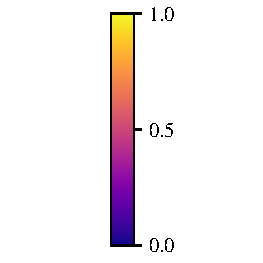
\includegraphics[width=0.3\textwidth]{papers/cahnhilliard/presentation/images/colorbar.book.pdf}}
\begin{subfigure}{0.3\textwidth}
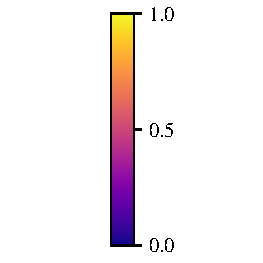
\includegraphics[width=\textwidth]{papers/cahnhilliard/presentation/images/colorbar.book.pdf}
\caption{Farbskala}
\end{subfigure}
\caption[Simulation der angepassten Cahn-Hilliard-Gleichung]{%
Anfangsbedingung $c(x,0)$ und
Simulationsresultate $c(x,1000\tau)$ von \eqref{cahnhilliard:acheq}
mit unterschiedlichen Rührstärken $\alpha$.}
\label{cahnhilliard:fig:achsim}
\end{figure}
